\section{State of the art}

Many nonlinear DR techniques and big data solutions discovered in recent years have lead to our divide-and-conquer proposal. Hence, we shall first review them to understand the advances they have achieved. In Section \ref{sec:DR-techniques}, our goal is to review four dimensionality reduction techniques that we will later apply our divide-and-conquer framework to. Next, in Section \ref{sec:MDS-big-data}, we will showcase in more detail the work of \citet{Delicado2024} with respect to classical MDS in big data to motivate our choosing of the divide-and-conquer approach. Finally, Sections \ref{sec:landmark-Isomap-OOC-DR-framework} and \ref{sec:openTSNE} offer a discussion about three more solutions to the big data problem in DR and how they relate to our proposal: landmark Isomap (\cite{Silva2002}), the out-of-core dimensionality reduction framework (\cite{Reichmann2024}) and novel Python t-SNE implementations.

\subsection{A few dimensionality reduction techniques}
\label{sec:DR-techniques}

\subsubsection{Non-classical MDS: the SMACOF algorithm}

SMACOF (Scaling by MAjorizing a COmplicated Function) is a multidimensional scaling procedure that minimizes metric stress using a majorization technique (\cite{Kruskal1964a,Kruskal1964b}). Given the distance matrix $\mathbf{D} = (\delta_{ij})$ of the original high-dimensional data and its corresponding low-dimensional distance matrix $\mathbf{D}_{\mathbf{\tilde{Y}}} = (d_{ij})$, metric stress determines how much different $\mathbf{D}$ and $\mathbf{D}_{\mathbf{\tilde{Y}}}$ are by the expression
$$
STRESS_M(\mathbf{D}, \mathbf{D}_{\mathbf{\tilde{Y}}}) = \sqrt{\frac{\sum_{i<j}\left(\delta_{i j}-d_{i j}\right)^2}{\sum_{i<j} \delta_{i j}^2}}.
$$
SMACOF (see Algorithm \ref{alg:SMACOF}) is faster for this problem than general optimization methods, such as gradient descent, and it consists on iterative Guttman transformations \citep{Guttman1968} applied to the embedded data.

\begin{algorithm}
    \caption{SMACOF}
    \label{alg:SMACOF}
    
    \begin{algorithmic}[1]
    \REQUIRE $\mathbf{D} = (\delta_{ij})$, the $n\times n$ matrix of observed distances; $q$, the embedding's dimensionality; $n\_iter$, the maximum number of iterations; and $\varepsilon$, the convergence threshold.
    \ENSURE $\boldsymbol{\mathbf{\tilde{Y}}}$, a configuration in a $q$-dimensional space.
    \STATE Initialize at random $\boldsymbol{\mathbf{\tilde{Y}}}^{(0)} \in \mathbb{R}^{n \times q}$
    \STATE $k \leftarrow 0$
    \REPEAT
        \STATE Compute the distance matrix of $\boldsymbol{\mathbf{\tilde{Y}}}^{(k)}$, $\mathbf{D}_{\boldsymbol{\mathbf{\tilde{Y}}^{(k)}}}$, with entries $d_{ij}^k = \|\tilde{y}_i^{(k)} - \tilde{y}_j^{(k)}\|$
        \STATE Compute the metric stress: $STRESS_M( \mathbf{D}, \mathbf{D}_{\boldsymbol{\mathbf{\tilde{Y}}^{(k)}}} )$
        \STATE Compute the Guttman transform: $\boldsymbol{\mathbf{\tilde{Y}}}^{(k+1)} = n^{-1}\mathbf{B}(\boldsymbol{\mathbf{\tilde{Y}}}^{(k)})\boldsymbol{\mathbf{\tilde{Y}}}^{(k)}$ where $\mathbf{B}(\boldsymbol{\mathbf{\tilde{Y}}}^{(k)}) = (b_{ij}^k)$:
        $$
        b_{ij}^k =
        \begin{cases}
        -\delta_{ij}/d_{ij}^k & \text{if } i \neq j \text{ and } d_{ij}^k > 0 \\
        0 & \text{if } i \neq j \text{ and } d_{ij}^k = 0 \\
        -\sum_{j \neq i} b_{ij}^k & \text{if } i = j
        \end{cases}
        $$
        \STATE $k \leftarrow k + 1$
    \UNTIL{$k \geq n\_iter$ or $|STRESS_M(\mathbf{D}, \mathbf{D}_{\mathbf{\tilde{Y}}^{(k-1)}}) - STRESS_M(\mathbf{D}, \mathbf{D}_{\mathbf{\tilde{Y}}^{(k)}})| < \varepsilon$}
    \RETURN $\boldsymbol{\mathbf{\tilde{Y}}}^{(k)}$
    \end{algorithmic}
\end{algorithm}

\subsubsection{LMDS}

Local multidimensional scaling (LMDS) is a variant of non-classical multidimensional scaling that differs in how large distances are treated \citep{Chen2009}. Specifically, a repulsive term between distant points is added to the stress function to further separate points in the low-dimensional configuration (see Algorithm \ref{alg:LMDS}). Parameters $\tau$ (which must be in the unit interval) and $k$ may be tuned with $k'$-cross validation thanks to the LC (Local Continuity) meta-criteria \citep{Chen2009}.

\begin{algorithm}
    \caption{LMDS}
    \label{alg:LMDS}
    
    \begin{algorithmic}[1]
    \REQUIRE $\mathbf{D} = (\delta_{ij})$, the $n \times n$ matrix of observed distances; $q$, the embedding's dimensionality; $k$, the size of neighborhoods; and $\tau$, the weight of the repulsive term.
    \ENSURE $\mathbf{\tilde{Y}}$, a configuration in a $q$-dimensional space.
    \STATE Compute the symmetrized $k$-NN graph of $\mathbf{D}$, $\mathcal{N}_k$
    \STATE Calculate $t=\frac{|\mathcal{N}_k|}{\left|\mathcal{N}_k^C\right|} \cdot \operatorname{median}_{\mathcal{N}_k}\left(\delta_{ij}\right) \cdot \tau$
    \STATE Minimize the modified stress function:
    $$
    \mathbf{\tilde{Y}} = \min_{\mathbf{Y} \in \mathbb{R}^{n\times q}} \sum_{(i, j) \in \mathcal{N}_k}\left(\delta_{ij}-\left\|\mathbf{y}_i-\mathbf{y}_j\right\|\right)^2 - t \sum_{(i, j) \notin \mathcal{N}_k}\left\|\mathbf{y}_i-\mathbf{y}_j\right\|
    $$
    \RETURN $\mathbf{\tilde{Y}}$
    \end{algorithmic}
\end{algorithm}

\subsubsection{Isomap}

Isomap \citep{Tenenbaum2000} is a nonlinear technique that preserves geodesic distances between points in a manifold (see Algorithm \ref{alg:Isomap}). The key insight of Isomap is that large distances between objects are estimated from the shorter ones by the shortest path length. Then, shorter and estimated-larger distances have the same importance in a final classical MDS step.

The only tuning parameter of Isomap is the bandwidth, which can be interpreted as the limiting distance of nearest neighbors, $\varepsilon$,  or the amount of nearest neighbors per point, $k$. However, there is no consensus on what is the best method to choose it.

\begin{algorithm}
    \caption{Isomap}
    \label{alg:Isomap}

    \begin{algorithmic}[1]
    \REQUIRE $\mathbf{D}$, the $n \times n$ matrix of observed distances; $q$, the embedding's dimensionality; and $\varepsilon$, the limiting distance of nearest neighbors, or $k$, the amount of nearest neighbors per point.
    \ENSURE $\mathbf{\tilde{Y}}$, a configuration in a $q$-dimensional space.
    \STATE Find the graph $\mathcal{N}$ given by the radius $\varepsilon>0$ or the $k$-NN
    \STATE Compute the distance matrix of $\mathcal{N}$, $\mathbf{D}_{\mathcal{N}}$
    \STATE Apply classical MDS to $\mathbf{D}_{\mathcal{N}}$: $\mathbf{\tilde{Y}} = \operatorname{MDS}(\mathbf{D}_{\mathcal{N}}, q)$
    \RETURN $\mathbf{\tilde{Y}}$
    
    \end{algorithmic}
\end{algorithm}

\subsubsection{t-SNE}

t-distributed stochastic neighbor embedding (t-SNE) is a nonlinear dimensionality reduction technique that preserves local neighborhoods by modeling similarities between points as conditional probabilities \citep{Vandermaaten2008}. The difference between these probability distributions in high and low-dimensional spaces is then minimized (see Algorithm \ref{alg:tSNE}).

t-SNE focuses on retaining the local structure of the data while ensuring that every point $\mathbf{y}_i$ in the low-dimensional space will have the same number of neighbors, making it particularly effective for visualizing clusters. The use of the Student's $t$ distribution with 1 degree of freedom (or Cauchy distribution) in the low-dimensional space addresses the \textit{crowding problem} by allowing dissimilar points to be modeled far apart (\cite{Vandermaaten2008}). The characteristic parameter of t-SNE is the perplexity, which can be interpreted as the average effective number of neighbors of the high-dimensional datapoints $\mathbf{x}_i$. Typical values are between 5 and 50.

\begin{algorithm}
    \caption{t-SNE}
    \label{alg:tSNE}
    
    \begin{algorithmic}[1]
    \REQUIRE $\mathbf{D} = (\delta_{ij})$, the $n \times n$ matrix of observed distances; $q$, the embedding's dimensionality; $Perp$, the perplexity.
    \ENSURE $\mathbf{\tilde{Y}}$, a configuration in a $q$-dimensional space.
    \STATE For every point $\mathbf{x}_i$, find $\sigma_i > 0$ so that the conditional probability ditribution
        $$
        p_{j|i} = \frac{\exp(-\delta_{ij}^2/2\sigma_i^2)}{\sum_{k \neq i}\exp(-\delta_{ik}^2/2\sigma_i^2)}\text{ if } i \neq j, \, p_{i|i} = 0
        $$ has perplexity $ Perp = 2^{-\sum_{j} p_{j|i} \log_2 p_{j|i}} $
    \STATE Symmetrize conditional distributions: $p_{ij} = \frac{p_{j|i} + p_{i|j}}{2n}$
    \STATE Consider Cauchy-distributed joint probabilities for the low-dimensional data $\mathbf{y}_i$: $$q_{ij} = \frac{(1 + \|y_i-y_j\|^2)^{-1}}{\sum_{h \neq k}(1 + \|y_h-y_k\|^2)^{-1}}$$
    \STATE Minimize the sum of Kullback-Leibler divergences between the joint distributions over all datapoints: $$
    \mathbf{\tilde{Y}} = \min_{\mathbf{Y} \in \mathbb{R}^{n\times q}} \sum_i \sum_j p_{j \mid i} \log \frac{p_{j \mid i}}{q_{j \mid i}}
    $$
    \RETURN $\mathbf{\tilde{Y}}$
    
    \end{algorithmic}
\end{algorithm}

\subsection{Multidimensional scaling for big data}
\label{sec:MDS-big-data}

\citet{Delicado2024} compared four existing versions of MDS with two newly proposed (divide-and-conquer MDS and interpolation MDS) to handle large datasets. As can be seen in Figure \ref{fig:bigmds}, these can be grouped into four categories:

\begin{itemize}
    \item \textbf{Interpolation-based}: landmark MDS, interpolation MDS and reduced MDS apply classical multidimensional scaling to a subset of $l \ll n$ points and then interpolate the projection of the remaining data. They differ in how the interpolation is computed: landmark MDS uses distance-based triangulation; interpolation MDS, the $l$-points Gower interpolation formula; and reduced MDS, the 1-point Gower interpolation formula.
    \item \textbf{Approximation-based}: pivot MDS approximates the SVD of the full inner product matrix with the SVD of the inner product matrix between a subset of $l \ll n$ points and all the points in the dataset.
    \item \textbf{Divide-and-conquer}: In divide-and-conquer MDS, the dataset is randomly partitioned into subsets of up to $l \ll n$ points into which MDS is independently applied. Then, the resulting embeddings are aligned with Procrustes transformations.
    \item \textbf{Recursive}: fast MDS is similar in spirit to divide-and-conquer MDS, but it partitions the data recursively. 
\end{itemize}

\begin{figure}
    \centering
    \captionsetup[subfigure]{labelformat=empty}

    \begin{subfigure}[t]{0.3\textwidth}
        \centering
        \includegraphics[width=.7\textwidth]{figures/landmark_MDS.png}
        \caption{landmark MDS}
        \label{fig:landmark_MDS}
    \end{subfigure}
    \hfill
    \begin{subfigure}[t]{0.3\textwidth}
        \centering
        \includegraphics[width=.7\textwidth]{figures/interpolation_adac.png}
        \caption{interpolation MDS}
        \label{fig:interpolation_MDS}
    \end{subfigure}
    \hfill
    \begin{subfigure}[t]{0.3\textwidth}
        \centering
        \includegraphics[width=.7\textwidth]{figures/reduced_MDS.png}
        \caption{reduced MDS}
        \label{fig:reduced_MDS}
    \end{subfigure}

    \begin{subfigure}[t]{0.3\textwidth}
        \centering
        \includegraphics[width=.7\textwidth]{figures/pivot_MDS.png}
        \caption{pivot MDS}
        \label{fig:pivot_MDS}
    \end{subfigure}
    \hfill
    \begin{subfigure}[t]{0.3\textwidth}
        \centering
        \includegraphics[width=.7\textwidth]{figures/divide_conquer_adac.png}
        \caption{divide-and-conquer MDS}
        \label{fig:divide_conquer_MDS}
    \end{subfigure}
    \hfill
    \begin{subfigure}[t]{0.3\textwidth}
        \centering
        \includegraphics[width=.9\textwidth]{figures/fast_adac.png}
        \caption{fast MDS}
        \label{fig:fast_MDS}
    \end{subfigure}
    
    \caption{Schematic representation of the six MDS algorithms for big data described in \cite{Delicado2024} (Source: original publication).}
    \label{fig:bigmds}
\end{figure}

\subsection{Landmark Isomap and the out-of-core dimensionality reduction framework}
\label{sec:landmark-Isomap-OOC-DR-framework}

\citet{Silva2002} first introduced landmark MDS as a step in landmark Isomap, a variation of Isomap that reduced the time complexity from $\mathcal{O}(n^3)$ to $\mathcal{O}(n^2l)$, where $l \ll n$ is the amount of landmark points. Other big data versions of MDS can be used with Isomap similarly. Nonetheless, interpolation-based and approximation-based algorithms cannot be trivially generalized to other nonlinear dimensionality reduction methods because they depend on the eigendecomposition computed in classical MDS.

Later, \citet{Reichmann2024} proposed the out-of-core dimensionality reduction framework. Similar to interpolation MDS, this algorithm applies a DR method that produces a mapping between high- and low-dimensional spaces (i.e. PCA, MDS, t-SNE, UMAP, autoencoders) to a small subset of the data and then projects the remaining datapoints in blocks. In order to obtain the aforementioned mappings, \citet{Reichmann2024} gathered a different projection mechanism for every method. PCA and autoencoders learn a parametric mapping between the original data and the embedding, so projecting new points is straightforward. For non-classical MDS, stress is minimized for a single point while keeping others fixed, a process known as \textit{single scaling} in the literature (\cite{Basalaj1999}). A similar strategy is used for t-SNE (\cite{Zhang2021}) and UMAP (\cite{McInnes2018a}), which leverage the k-NN of the projecting point to initialize the optimizer.

\subsection{openTSNE, an outstanding implementation of t-SNE}
\label{sec:openTSNE}

Maybe because of its popularity, t-SNE has been optimized for large data environments in Python through iterative implementations. \citet{Policar2024} considered many of them and published \verb|openTSNE|, a package that includes several t-SNE extensions \enquote{\textit{to address scalability issues and the quality of the resulting visualizations}}. Furthermore, they compared their proposal with those of other popular packages in serial and parallel configurations. In Figure \ref{fig:python_tsne_benchmarks} it can be seen that, thanks to these advances, the challenges of big data have already been solved in the specific case of t-SNE.

\begin{figure}
    \centering
    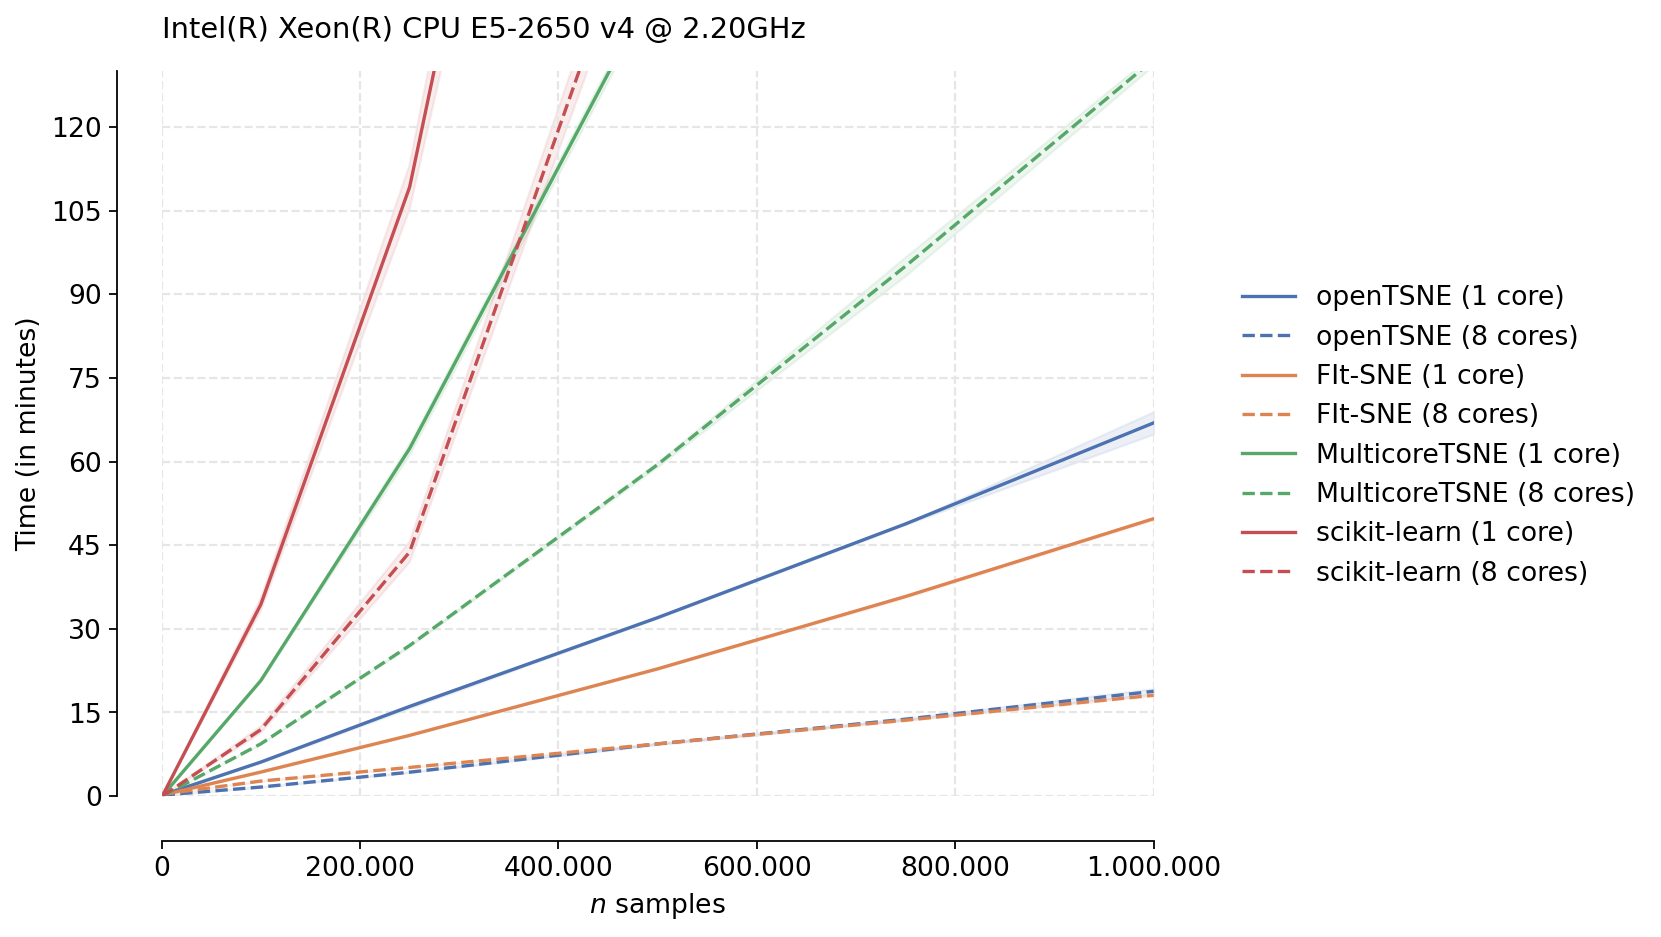
\includegraphics[width=0.8\textwidth]{figures/python_tsne_benchmarks.png}
    \caption{Benchmark of the best open-source t-SNE Python implementations by \citet{Poličar2023} (Source: original webpage).}
    \label{fig:python_tsne_benchmarks}
\end{figure}